\chapter{State Estimation}
\label{ch:estimation}
The SSCPAC robotics group has developed the Autonomous Capabilities Suite (ACS) which incorporates many different robotics related algorithms into a single software package that can be run on a wide variety of robots and is able to easily accomodate different payload and sensor suites \cite{Sights06}. One of the ACS libraries is the adaptive extended Kalman filter which is used on the EOD robots for state estimation and is the main method used for answering the question ``Where am I?''. The idea behind the Kalman filter is relatively straightforward in that the robot has some basic idea of where it is in the world using its sensors but there is uncertainty involved in that estimate due to:
\begin{itemize}
\item different measurement accuracies from the sensors,
\item multiple sensors measuring the same state,
\item some states that are not measured,
\item imperfect models of the robot dynamics.
\end{itemize}

The Kalman filter is a method to merge physical models and sensor data to come up with a better estimate of where the robot is located, what its orientation is and how fast it is moving than any of the sensors measure on their own. There are four models used in the Kalman filter:
\begin{itemize}
\item system model based on physics,
\item measurement model to transform sensor output to state coordinate system,
\item system noise model,
\item measurement noise model.
\end{itemize}

%*** Put in a picture of the PackBot driving with one track going over two-by-fours. ***

%*** May want to use the example from the KF presentation instead of this example. I could use better images that way as well. ***

%An example is trying to determine the heading of a robot that is driving in a straight line where the left track is moving on a flat surface while the right track is moving on an uneven surface as in Figure \ref{fig:topology}. The wheel encoders measure the distance traveled by each track and will report that the right track is traveling a greater distance than the left track which could mean that (a) the robot is turning counter-clockwise or (b) the robot tracks are moving over different surface topologies. At the same time the robot will be getting measurements about its heading from both the IMU and GPS sensors where each of those sensors will have some noise as well. As long as the controller is performing adequately and the robot is indeed traveling in a straight line with a constant heading then the IMU and GPS sensor measurements would likely indicate that the robot is traveling in a straight line. The job of the Kalman filter is to determine how much to trust the IMU, GPS and wheel encoders when calculating the robot heading and to give an accurate estimate of the actual state of the robot at any given time, especially in situations like this example where there are possible conflicting measurements.

%\begin{figure}[ht!]
%	\centering
%	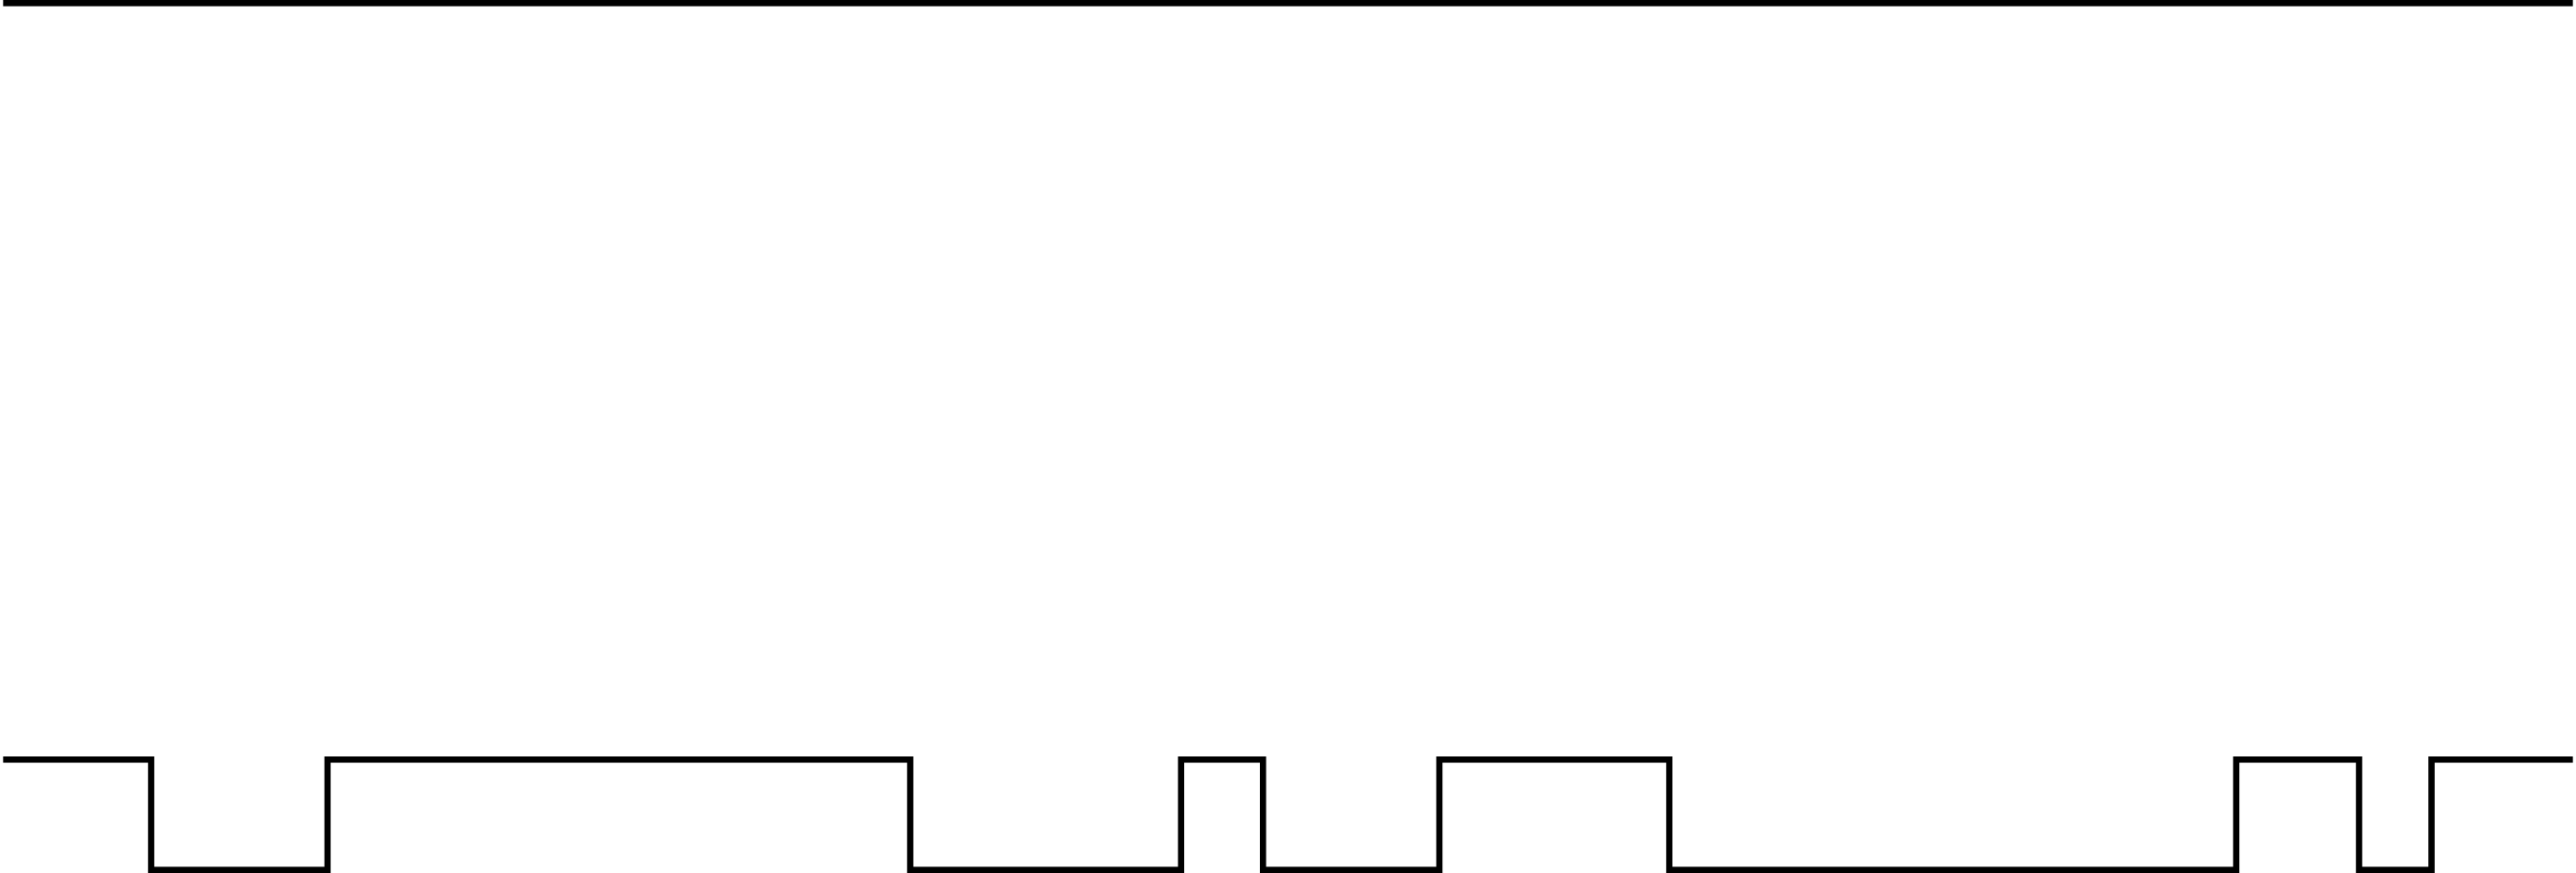
\includegraphics[width=.5\textwidth]{images/topography}
%	\caption{Different topologies for the left track and the right track when the ground is smooth on the left side and bumpy on the right side. The top line is for the left track and the bottom line is for the right track. The right track travels a greater distance than the left track.}
%	\label{fig:topology}
%\end{figure}

\section{State Space Models}
\label{sec:statespacemodels}
Kalman filters and modern control systems (see Chapter \ref{ch:controls}) use the idea of a multi-dimensional state space to encapsulate all of the relevant information that is known about a system. In the case of robots like the ones used in these experiments the states of interest are position, orientation and linear and angular velocities. In general a system is described by nonlinear equations that describe how the state variables change through time and how measurements of the system are related to the states as given by

\begin{align}
\label{eq:statespace}
\begin{split}
\dot{x} &= f(x,u,t) \\
\dot{y} &= h(x,t).
\end{split}
\end{align}

The state variables are given in vector form by $x$ and the sensor measurements are contained in the vector $y$. The state space equations are a means of representing with compact notations how the state of a system changes through time based on the initial state of the system and the inputs to the system, $u$, which allows the trajectory (or motion through time) to be calculated. The inputs are assumed to include any external forces applied to the system as well as actuation provided by the system itself. The function $h(x,t)$ transforms the sensor measurements into state variables which is important when the units of a sensor are not the same as the units of the state.

For the robots used in these experiments the state vector used follows that found in \cite{Kelly_1994_338}, \cite{Kelly_1994_333} where the state variables are

\begin{align*}
x_k = \left[\begin{array}{c c c c c c c c} x & y & z & V & \theta & \phi & \psi & \omega \end{array}\right]^T.
\end{align*}
In this vector $x$, $y$ and $z$ are positions, $V$ is linear velocity, $\theta$, $\phi$ and $\psi$ are Euler angles for pitch, roll and yaw, and $\omega$ is angular velocity as shown in Figure \ref{fig:packbotaxes}.

\begin{figure}[ht!]
    \centering
    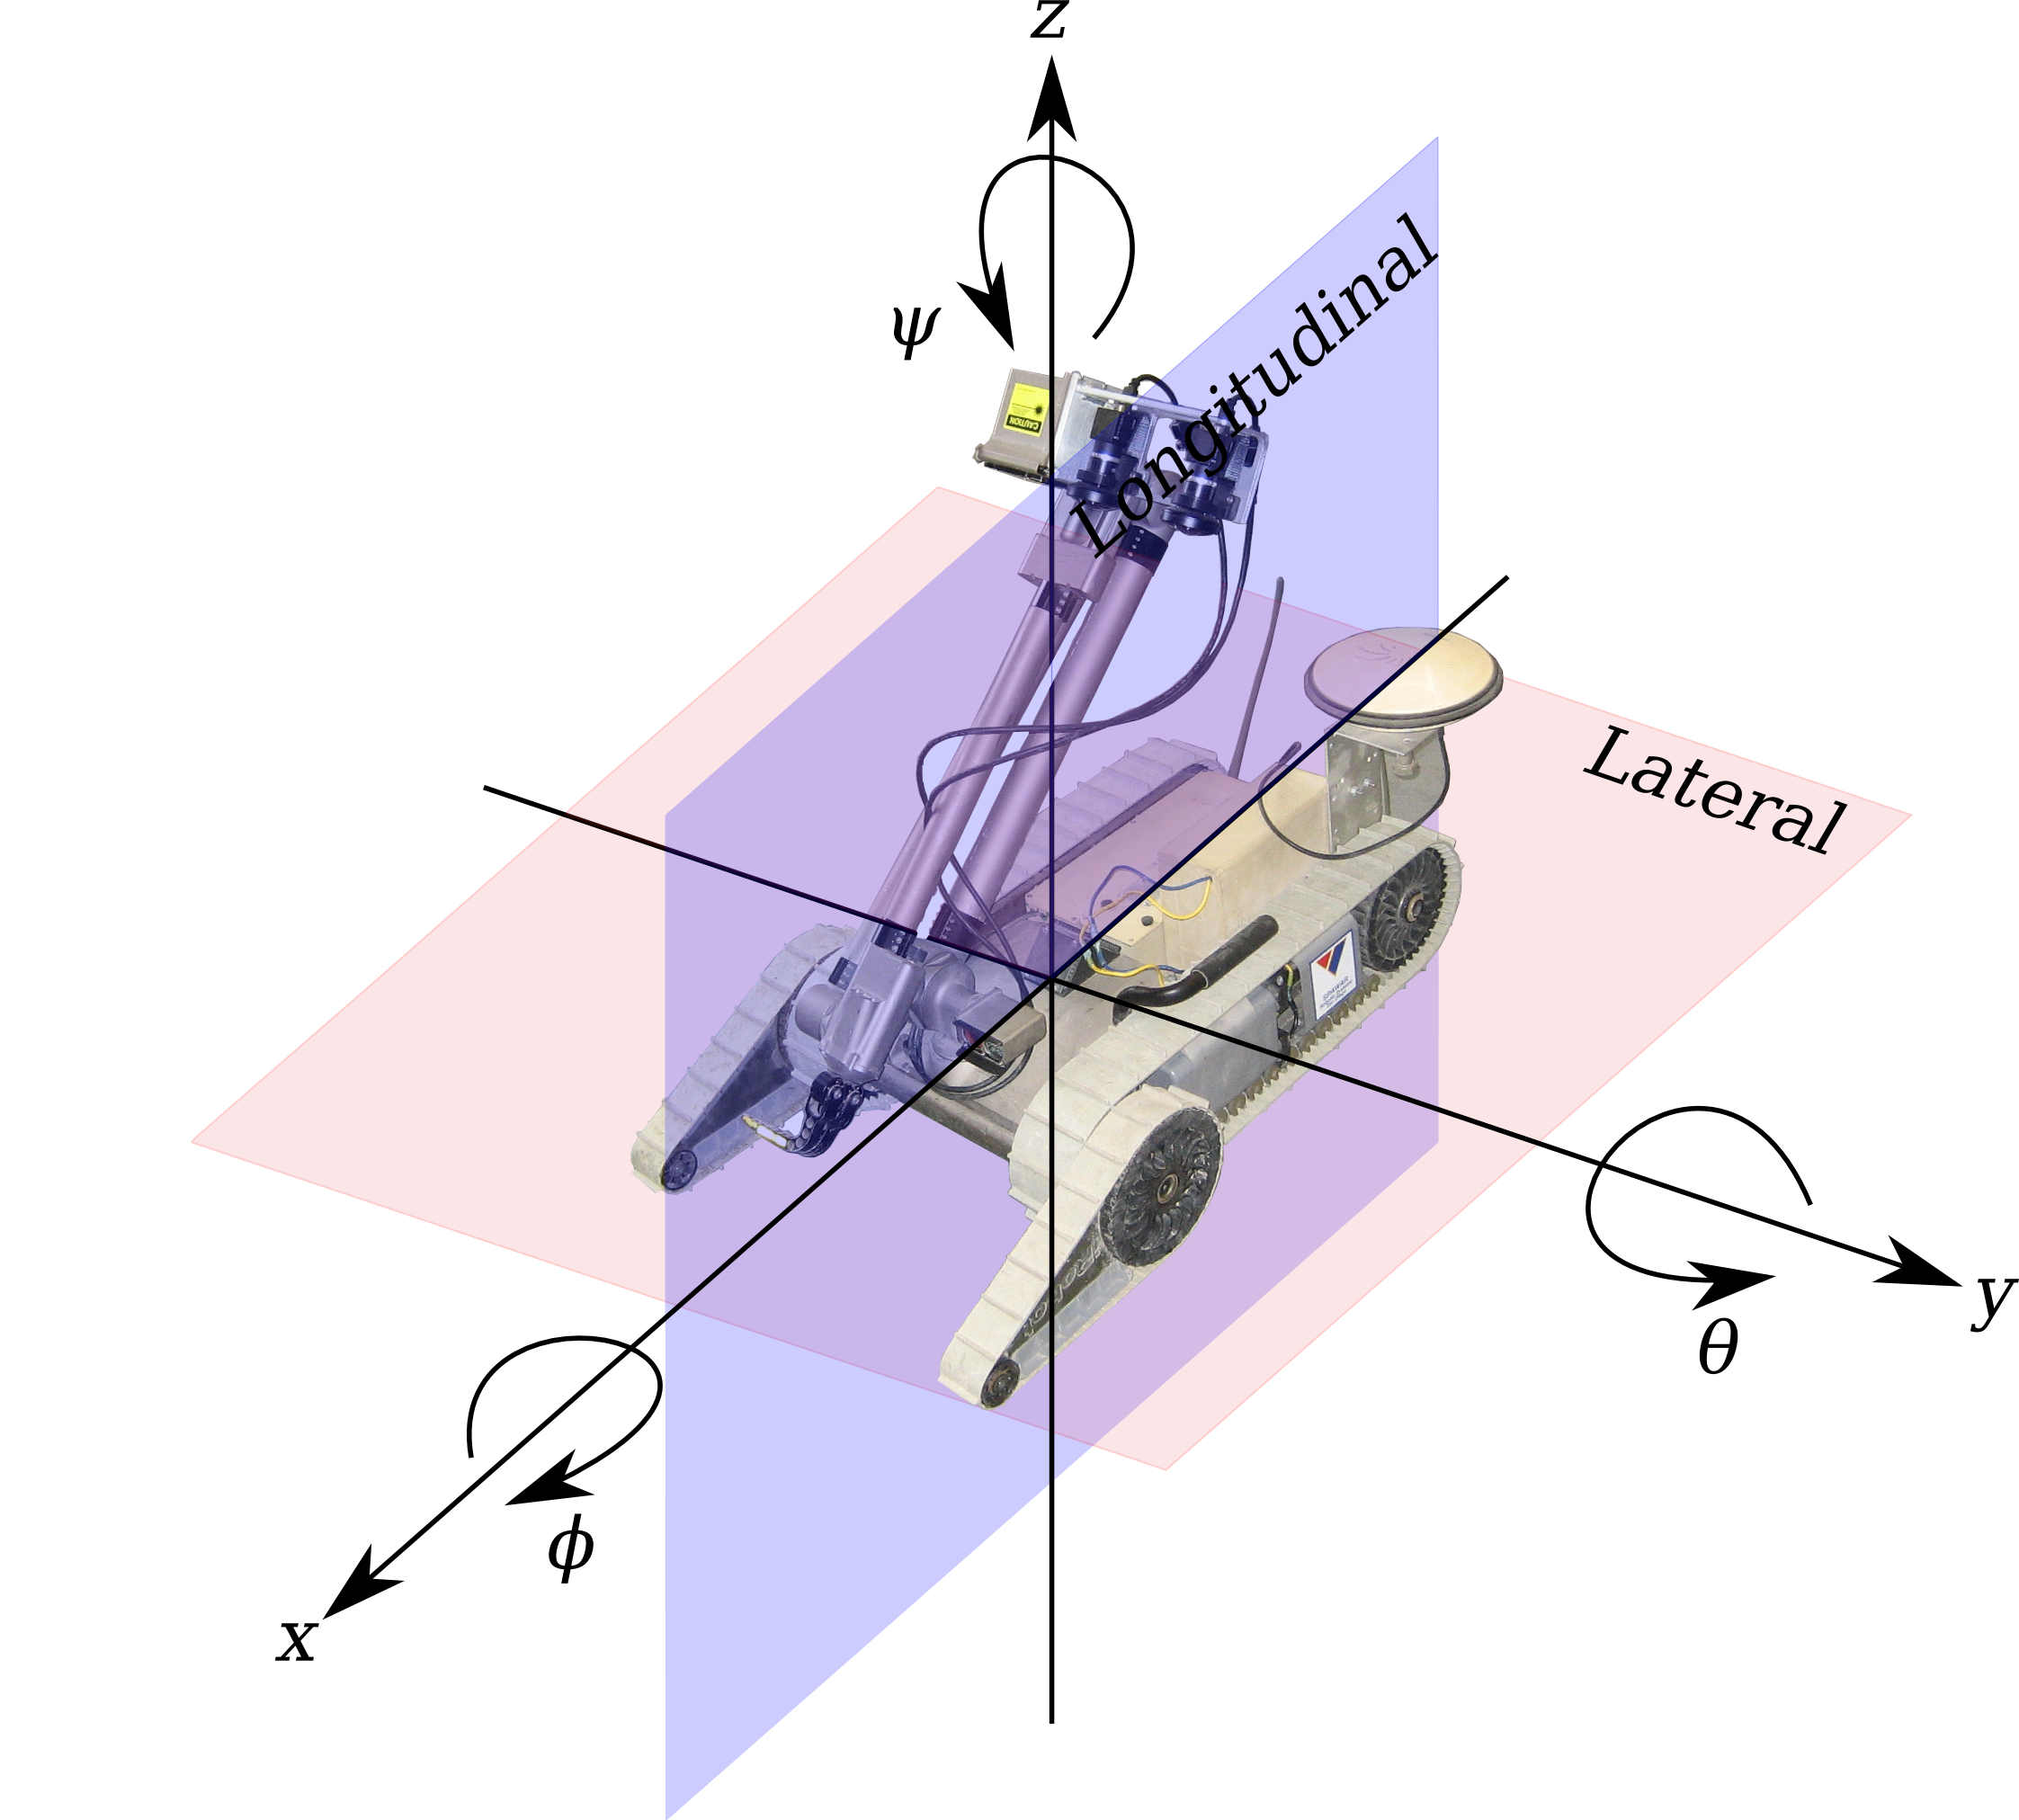
\includegraphics[width=.8\textwidth]{images/packbotaxes}
    \caption{PackBot used in experiments with axes for position and orientation shown.}
    \label{fig:packbotaxes}
\end{figure}

\section{The Kalman Filter}
\label{sec:kalmanfilter}
The ACS Kalman filter is typical of all Kalman filters in that it consists of a prediction update step and a measurement update step where the prediction update is run as fast as possible and the measurement update is run whenever new sensor data becomes available as in Figure \ref{fig:kf}. The prediction update step uses a model of the system dynamics and a measurement of elapsed time to determine where the system is in the world and will inevitably have errors. Some of the errors are due to effects that are not captured in the models, (im)precision of the clock on the computer for measuring time and simplifying assumptions that are made in order to be able to calculate the system model in real-time using embedded computers. The measurement update step is basically a feedback step to help correct for errors in the system model using sensors to provide current data \cite{Kelly_1994_338}.

\begin{figure}[ht!]
	\centering
	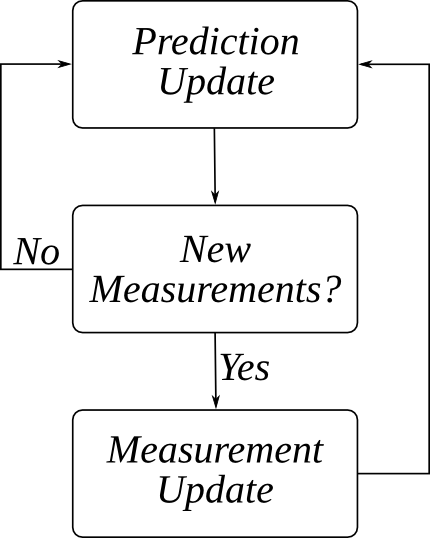
\includegraphics[width=.4\textwidth]{images/kf}
	\caption{The Kalman filter algorithm.}
	\label{fig:kf}
\end{figure}

The Kalman filters that run on the small UGVs used in these experiments run on digital computers and are necessarily used in discrete time rather than continuous time because of the nature of computers. Additionally, the standard Kalman filter equations make the assumption that the system and measurement models are linear. From \cite{Kelly_1994_338}, \cite{Simon06OptimalEstimation} the discretized and linearized versions of (\ref{eq:statespace}) mean that the state space equations are represented as

\begin{align}
\label{eq:kfstatemodel}
\begin{split}
x_{k+1} &= \Phi_kx_k + w_k \\
y_k &= H_kx_k + v_k
\end{split}
\end{align}
where $\Phi_k$ is the state transition matrix relating the state at time $k+1$ to time $k$ in the absence of inputs or noise and models the system dynamics, $w_k$ is system noise due to an imperfect model, $H_k$ is the measurement matrix which relates the measurements to the state vector and $v_k$ is the sensor measurement noise. The Kalman filter uses an unforced model so all inputs are considered disturbances to the steady-state dynamics. This means that $w_k$ includes noise, modeling errors, external forces and actuator forces.

The prediction update step marches the system dynamics forward in time using the equations

\begin{align}
\label{eq:kfpredictionupdate}
\begin{split}
\hat{x}_{k+1}^- &= \Phi_k\hat{x}_k^+ \\
P_{k+1}^- &= \Phi_kP_k^+\Phi_k^T + Q_k
\end{split}
\end{align}
and the measurement update step provides feedback from sensor data using the equations

\begin{align}
\label{eq:kfmeasurementupdate}
\begin{split}
K_k &= P_k^-H_k^T\left[H_kP_k^-H_k^T + R_k\right]^{-1} \\
\hat{x}_k^+ &= \hat{x}_k^- + K_k\left[y_k - H_k\hat{x}_k^-\right] \\
P_k^+ &= \left[I - K_kH_k\right]P_k^-.
\end{split}
\end{align}
where $P_k$ is the state covariance matrix, $K_k$ is the Kalman gain, $Q_k$ is the process covariance matrix giving a measure of the expected noise in the system model and $R_k$ is the measurement covariance matrix giving the expected noise of the sensors. Using (\ref{eq:kfpredictionupdate}) and (\ref{eq:kfmeasurementupdate}) an estimate of the state of the robot can be obtained at any time for use by the controls algorithms or to give feedback to a human operator.

*** Somewhere, maybe here, I want to say that $P_k$ is a measure of how good the state estimate is likely to be and that the gain $K_k$ weights whether the state estimate is based on the system model or the measurements. The gain $K_k$ is a function of the process and measurement covariance matrices so it really matters how those variances are set up relative to one another more than that they are absolutely correct values. ***

The variables $\hat{x}_k^-$ and $\hat{x}_k^+$ in (\ref{eq:kfpredictionupdate}) and (\ref{eq:kfmeasurementupdate}) refer to estimates of the state variables before and after the measurement update step in the Kalman filter, respectively.

\subsection{Models in the Kalman Filter}
\label{sec:kfModels}
The Kalman filter relies on several models that are used to determine estimates of the states for a system. The ACS Kalman filter uses four such models:

\begin{itemize}
\item System dynamics model,
\item measurement model,
\item system noise model,
\item measurement noise model.
\end{itemize}

It is important to recognize that the interaction between these four models determines how well the Kalman filter output will represent the true state of the robot.

\subsection{Assumptions in the System Model}
\label{sec:kfAssumptions}
It is nearly impossible to develop models that completely capture all of the attributes of most systems, including robots that are expected to operate in many different physical environments, so assumptions are made to simplify the system model. The following assumptions allow the prediction update step to be calculated in a reasonable amount of time using modern computers so that a state estimate is available that the control systems can act upon in real time. The assumptions also allow a single system model to be abstracted and used on multiple similar but different robotic vehicles.

\subsubsection{Low Dynamics Assumption}
\label{sec:kfLowDynamicsAssumption}
The first assumption made is that, from one time step to the next, the robot will not be accelerating fast enough in any direction for the sensors on the robot to be able to measure the accelerations. This means that the two velocities, linear and angular, in the state vector will be assumed to be constant. The benefit of this assumption is that there are six fewer states that must be tracked in the state vector, one for acceleration about each axis of the robot.

\subsubsection{Principal Motion Assumption}
\label{sec:kfPrincipalMotionAssumption}
The second assumption says that, during a single time step, the position of the robot will only be a function of linear velocity and the orientation of the robot will only be a function of the angular velocity. Figure \ref{fig:packbotaxes} helps in visualizing the effect of rotating the robot about its center and how that will not affect the position of the robot. This assumption allows several terms in the system model to be set to zero.

\subsection{Continuous to Discrete Time Transform}
\label{sec:kfContToDiscTransform}
The system model will be developed using continuous time nonlinear differential equations but the Kalman filter on the robots will be running on digital computers so the model will need to be converted to discrete time. In continuous time the system model will be

\begin{align*}
\dot{x} = Fx
\end{align*}
and in discrete time the system model will be

\begin{align*}
x_{k+1} = \Phi_k x_k.
\end{align*}
The transformation from continuous to discrete time obeys an exponential matrix transformation with a Taylor series approximation \cite{Gopal93} given by

\begin{align*}
\Phi_k = e^{F\Delta_T} = I + F\Delta_T + \frac{(F\Delta_T)^2}{2!} + \ldots + \frac{(F\Delta_T)^n}{n!}
\end{align*}
A first order Taylor series approximation is good enough if the nonlinearities in the system are small enough and in the case of the robots used in these experiments that is assumed to be the case so the transformation used is simply

\begin{align}
\label{eq:kfContToDiscTransform}
\Phi_k = I + F\Delta_T.
\end{align}

\subsection{System Dynamics Model}
\label{sec:dynamics}
A model of the system dynamics is necessary in order to propagate the state of the system forward in time in the absence of measurements. It is impossible to create a perfect model of the system and even a nearly perfect model of the system will likely be too complex to compute fast enough for it to be useful. The best result that is typically available is a model with a large amount of assumptions where the most important aspects of the dynamics are captured in the model.

A nonlinear, continuous time model based on robot kinematics is developed in the body frame coordinate system using the states from \S\ref{sec:statespacemodels} is given by

\begin{align}
\label{eq:kfnonlineardynamics}
\begin{split}
\frac{d}{dt}\left[\begin{array}{c}
x \\ y \\ z \\ V \\ \theta \\ \phi \\ \psi \\ \omega
\end{array}\right] =
\left[\begin{array}{c}
V\cos\psi\cos\theta \\
V\sin\psi\cos\theta \\
-V\sin\theta \\
0 \\
-\omega\sin\phi \\
\omega\tan\theta\cos\phi \\
\omega\cos\phi/\cos\theta \\
0
\end{array}\right].
\end{split}
\end{align}

\subsection{Extended Kalman Filter}
\label{sec:extendedkf}
The basic Kalman filter makes the assumption that both the system model contained in $\Phi_k$ and the measurement model in $H_k$ are linear. The extended Kalman filter (EKF) allows for nonlinear models such as that given by (\ref{eq:kfnonlineardynamics}) to be used for $\Phi_k$, $H_k$ or both by linearizing the models around the state estimate. To linearize the models the Jacobian, or matrix of partial derivatives, is taken about the estimated state. The idea of linearization of a nonlinear model is shown in Figure \ref{fig:KFLinearization} where the linearization can be seen to be more accurate when the system nonlinearities are small meaning that the dynamics are slow.

\begin{figure}[ht!]
	\centering
    \subfloat[Slow dynamics.] {
	    \label{images/KFLinearizationSlow}
        \includegraphics[width=.3\textwidth]{images/KFLinearizationSlow}
    }
    \hfill
    \subfloat[Medium dynamics.] {
        \label{images/KFLinearizationMedium}
	    \includegraphics[width=.3\textwidth]{images/KFLinearizationMedium}
    }
    \hfill
    \subfloat[Fast dynamics.] {
        \label{images/KFLinearizationFast}
	    \includegraphics[width=.3\textwidth]{images/KFLinearizationFast}
    }
	\caption{Effects of linearizing a nonlinear model. Success depends on the speed of the dynamics, either \subref{images/KFLinearizationSlow} slow, \subref{images/KFLinearizationMedium} medium or \subref{images/KFLinearizationFast} fast.}
	\label{fig:KFLinearization}
\end{figure}

The nonlinear state dynamics were described in (\ref{eq:kfnonlineardynamics}). The Jacobian of that state vector equation is calculated using

%{\tiny
\begin{align*}
\dot{x} =
\underbrace{\left[\begin{array}{c c c c c c c c}
\frac{\partial \dot{x}}{\partial x} & \frac{\partial \dot{x}}{\partial y} & \frac{\partial \dot{x}}{\partial z} & \frac{\partial \dot{x}}{\partial V} & \frac{\partial \dot{x}}{\partial \theta} & \frac{\partial \dot{x}}{\partial \phi} & \frac{\partial \dot{x}}{\partial \psi} & \frac{\partial \dot{x}}{\partial \omega} \\
\frac{\partial \dot{y}}{\partial x} & \frac{\partial \dot{y}}{\partial y} & \frac{\partial \dot{y}}{\partial z} & \frac{\partial \dot{y}}{\partial V} & \frac{\partial \dot{y}}{\partial \theta} & \frac{\partial \dot{y}}{\partial \phi} & \frac{\partial \dot{y}}{\partial \psi} & \frac{\partial \dot{y}}{\partial \omega} \\
\frac{\partial \dot{z}}{\partial x} & \frac{\partial \dot{z}}{\partial y} & \frac{\partial \dot{z}}{\partial z} & \frac{\partial \dot{z}}{\partial V} & \frac{\partial \dot{z}}{\partial \theta} & \frac{\partial \dot{z}}{\partial \phi} & \frac{\partial \dot{z}}{\partial \psi} & \frac{\partial \dot{z}}{\partial \omega} \\
\frac{\partial \dot{V}}{\partial x} & \frac{\partial \dot{V}}{\partial y} & \frac{\partial \dot{V}}{\partial z} & \frac{\partial \dot{V}}{\partial V} & \frac{\partial \dot{V}}{\partial \theta} & \frac{\partial \dot{V}}{\partial \phi} & \frac{\partial \dot{V}}{\partial \psi} & \frac{\partial \dot{V}}{\partial \omega} \\
\frac{\partial \dot{\theta}}{\partial x} & \frac{\partial \dot{\theta}}{\partial y} & \frac{\partial \dot{\theta}}{\partial z} & \frac{\partial \dot{\theta}}{\partial V} & \frac{\partial \dot{\theta}}{\partial \theta} & \frac{\partial \dot{\theta}}{\partial \phi} & \frac{\partial \dot{\theta}}{\partial \psi} & \frac{\partial \dot{\theta}}{\partial \omega} \\
\frac{\partial \dot{\phi}}{\partial x} & \frac{\partial \dot{\phi}}{\partial y} & \frac{\partial \dot{\phi}}{\partial z} & \frac{\partial \dot{\phi}}{\partial V} & \frac{\partial \dot{\phi}}{\partial \theta} & \frac{\partial \dot{\phi}}{\partial \phi} & \frac{\partial \dot{\phi}}{\partial \psi} & \frac{\partial \dot{\phi}}{\partial \omega} \\
\frac{\partial \dot{\psi}}{\partial x} & \frac{\partial \dot{\psi}}{\partial y} & \frac{\partial \dot{\psi}}{\partial z} & \frac{\partial \dot{\psi}}{\partial V} & \frac{\partial \dot{\psi}}{\partial \theta} & \frac{\partial \dot{\psi}}{\partial \phi} & \frac{\partial \dot{\psi}}{\partial \psi} & \frac{\partial \dot{\psi}}{\partial \omega} \\
\frac{\partial \dot{\omega}}{\partial x} & \frac{\partial \dot{\omega}}{\partial y} & \frac{\partial \dot{\omega}}{\partial z} & \frac{\partial \dot{\omega}}{\partial V} & \frac{\partial \dot{\omega}}{\partial \theta} & \frac{\partial \dot{\omega}}{\partial \phi} & \frac{\partial \dot{\omega}}{\partial \psi} & \frac{\partial \dot{\omega}}{\partial \omega}
\end{array}\right]}_{F}
\left[\begin{array}{c}
x \\ y \\ z \\ V \\ \theta \\ \phi \\ \psi \\ \omega
\end{array}\right]
\end{align*}
%}
which results in

{\scriptsize
\begin{align}
\label{eq:kfjacobianresult}
\frac{d}{dt}\left[\begin{array}{c}
x \\ y \\ z \\ V \\ \theta \\ \phi \\ \psi \\ \omega
\end{array}\right] =
\underbrace{\left[\begin{array}{c c c c c c c c}
0 & 0 & 0 & c\psi c\theta & -V c\psi s\theta               & 0                     & -V s\psi c\theta & 0 \\
0 & 0 & 0 & s\psi c\theta & -V s\psi s\theta               & 0                     & V c\psi c\theta  & 0 \\
0 & 0 & 0 & -s\theta      & -V c\theta                     & 0                     & 0                & 0 \\
0 & 0 & 0 & 0             & 0                              & 0                     & 0                & 0 \\
0 & 0 & 0 & 0             & 0                              & -\omega c\phi         & 0                & -s\phi \\
0 & 0 & 0 & 0             & \omega c\phi/c^2\theta         & \omega t\theta s\phi  & 0                & t\theta c\phi \\
0 & 0 & 0 & 0             & \omega s\theta c\phi/c^2\theta & -\omega s\phi/c\theta & 0                & c\phi/c\theta \\
0 & 0 & 0 & 0             & 0                              & 0                     & 0                & 0
\end{array}\right]}_{F}
\left[\begin{array}{c}
x \\ y \\ z \\ V \\ \theta \\ \phi \\ \psi \\ \omega
\end{array}\right].
\end{align}
}
Applying the principal motion assumption to set the terms relating position and angular velocity as well as orientation and linear velocity to zero in addition to converting from continuous to discrete time to put ones on the diagonal gives

\begin{align}
\label{eq:kfSystemModelWithAssumptions}
x_{k+1} = 
\underbrace{\left[\begin{array}{c c c c c c c c}
1 & 0 & 0 & c\psi c\theta \Delta_T & 0 & 0 & 0 & 0 \\
0 & 1 & 0 & s\psi c\theta \Delta_T & 0 & 0 & 0 & 0\\
0 & 0 & 1 & -s\theta \Delta_T & 0 & 0 & 0 & 0\\
0 & 0 & 0 & 1 & 0 & 0 & 0 & 0 \\
0 & 0 & 0 & 0 & 1 & 0 & 0 & -s\phi \Delta_T \\
0 & 0 & 0 & 0 & 0 & 1 & 0 & t\theta c\phi \Delta_T \\
0 & 0 & 0 & 0 & 0 & 0 & 1 & c\phi \Delta_T/c\theta \\
0 & 0 & 0 & 0 & 0 & 0 & 0 & 1
\end{array}\right]}_{\Phi_k}
\left[\begin{array}{c}
x \\ y \\ z \\ V \\ \theta \\ \phi \\ \psi \\ \omega
\end{array}\right]_k
\end{align}
as the system model that is used in the prediction update step of the Kalman filter equations to calculate the state of the robot in between measurements.

\subsection{Measurement Model}
\label{sec:kfMeasurementModel}
The measurement model converts sensor data to the state variable coordinate system and for a standard sensor suite is by far the simplest model used in the ACS Kalman filter. The idea is that, for a sensor that measures one of the states, the data that is output by the sensor has to have the same units and be in the same range as the state variable. This is best illustrated by an example.

Suppose a compass and an IMU both measure the yaw state variable and the compass output is $0 - 360^\circ$ whereas the IMU output is $0 - 2\pi~rads$ and the yaw state in the Kalman filter is tracked in the range $0 - 2\pi$. If, for one time step, both compass and IMU measurements are available to be incorporated into the Kalman filter then the measurement update step from (\ref{eq:kfmeasurementupdate}) is run and the $H$ matrix is

\begin{align*}
H = \left[\begin{array}{c c c c c c c c}
0 & 0 & 0 & 0 & 0 & 0 & \frac{\pi}{180^\circ} & 0 \\
0 & 0 & 0 & 0 & 0 & 0 & 1 & 0
\end{array}\right].
\end{align*}

There is one row per sensor measurement and one column per state in the measurement matrix so in this example $H$ is a $2\times8$ matrix. The compass measurement corresponds to the first row and the data is converted from degrees to radians. The IMU measurement corresponds to the second row and, since the units of the sensor data are the same as the units of the state variable, the data is not transformed at all.

In the case when there is a single sensor measuring each of the states and those sensors output data that is in the correct units and range of the state variables then $H=I$.

\subsection{Noise Models}
\label{sec:kfNoiseModels}
The noise models attempt to estimate noise coming in from the terms in the equations

\begin{align*}
\begin{split}
x_{k+1} &= \Phi_kx_k + w_k \\
y_k &= H_kx_k + v_k
\end{split}
\end{align*}

The Kalman filter uses two different noise models, one for system noise $w_k$ and one for measurement noise $v_k$. The system noise model attempts to capture all of the effects due to an imperfect system model, linearization of the model, the low dynamics assumption and the principal motion assumption. The measurement noise model tries to compensate for sensors that do not model the environment perfectly.

Noise in the Kalman filter is assumed to be zero mean with a Gaussian distribution. The models are set up as covariance matrices that describe the Gaussian distribution of each of the noise terms for either the states or the sensors where the state noise model is given by $Q$ and the measurement noise model is given by $R$.

\subsection{Kalman Gain}
\label{kfKalmanGain}
The Kalman gain matrix is used in the measurement update step (\ref{eq:kfmeasurementupdate}) and essentially weights whether the state estimate will rely more on the system model or the measurements and is given by

\begin{align*}
K_k &= P_k^-H_k^T\left[H_kP_k^-H_k^T + R_k\right]^{-1}
\end{align*}

where

\begin{align*}
P_{k+1}^- &= \Phi_kP_k^+\Phi_k^T + Q_k.
\end{align*}

From these equations it can be seen that all four models used in the Kalman filter are used to calculate the Kalman gain matrix since $\Phi$, $Q$, $H$ and $R$ are all present. In the measurement update step the Kalman gain is multiplied by the difference between the measured values $y_k$ of the state and the expected values of those measurements based on the system model $\hat{y}_k$ where $\hat{y}_k = H\hat{x}_k^-$ is what the sensors would report if there were no noise in the measurements and the system model were perfect. The state estimate from the measurement update step is

\begin{align*}
\hat{x}_k^+ &= \hat{x}_k^- + K_k\left[y_k - H_k\hat{x}_k^-\right].
\end{align*}

If the sensor data matches the system model prediction then the term $y_k-H_k\hat{x}_k^-=0$ and the Kalman gain is ignored but that rarely, if ever, happens in practice. The interesting question then becomes whether to trust the noisy sensors or the imperfect system model to determine the state estimate. A large gain value will adjust the previous estimate from the prediction update step by a larger amount which means that the sensor data is weighted more heavily than the system model. Conversely a small gain value will cause the estimate from the measurement update step to trust the system model more than the sensor data. It is important to note that the Kalman gain matrix $K$ can have large values for some states (and sensors) and small values for other states (and sensors).

As discussed in \S\ref{sec:kfMeasurementModel} the measurement model is fairly simple so the Kalman gain is really a function of the system model and the noise models. If the system model is a very good approximation to the real system then the system noise model should reflect that by having small values in $Q$ and if the sensors are very good then the measurement noise model will have small values in $R$. Thus the Kalman gain matrix tends to take on values relative to the ratio of the elements of the $Q$ and $R$ noise models. From this it can be seen that developing accurate noise models is very important to the performance of the Kalman filter. When the noise models are not set up correctly then the state estimate covariance $P_K$ begins to grow larger.

\section{Establishing Ground Truth}
\label{sec:groundtruth}
Quantitatively evaluating the performance of Kalman filters can be accomplished in several ways, the best of which is to analyze the output of the Kalman filter against ground truth. Although it is nearly impossible to establish ground truth over a large area in practice the closer the measurements are to an absolute position in the world the better. To determine ground truth for the robots in these experiments a differential GPS (DGPS) system was created independently of the sensors on the robot so that very accurate measurements of the robots actual position could be logged and then used in a post-processing step to determine how well the Kalman filter estimate corresponds to ground truth.

The DGPS system consists of a GPS receiver and serial radio that make up the base station and a GPS receiver, serial radio and small computer that make up the roaming station as in Figure \ref{fig:dgps}. The GPS receivers are both Novatel receivers using the Real Time Kinematics algorithm. The base station is located in a static position and is configured to use a fixed position which is compared to what the current position would be if it were not fixed. The difference between the fixed position and the calculated position are used to generate corrections that would put the position of the GPS antenna at the fixed position and those corrections are sent to and applied at the roaming station resulting in a standard deviation of $2$ $cm$ for the position output of the roaming station. The errors are due to the effects of the GPS signal passing through the atmosphere from the satellites to the antenna as well as to multipath effects closer to the ground. The DGPS corrections are used for each satellite that the ground station and the roaming station share in the constellation of satellites they are using in their solution of a position estimate. The DGPS system is bootstrapped to the robot during testing runs to log data at a rate of $20$ $Hz$ and is only used as a tool to improve Kalman filter performance and is not meant to be used during normal operation.

With a highly accurate estimate of ground truth established it becomes possible to not only study the performance of the Kalman filter but to also begin determining whether to focus efforts in improving the autonomous navigation behaviors of the robots via the estimation or controls algorithms.

\begin{figure}[ht!]
	\centering
	\includegraphics[width=.6\textwidth]{images/dgps}
	\caption{Differential GPS system diagram.}
	\label{fig:dgps}
\end{figure}

\section{Identifying Noise Models}

\subsection{Adaptive Extended Kalman Filter}
\label{sec:adaptiveekf}
*** Discuss why $Q$ and $R$ are important and what function they serve in the Kalman filter. Why is it valid to update $Q$ and $R$ this way? Talk about how the updates are turned off when the velocity is zero, otherwise $Q$ and $R$ are adapted to a static, not dynamic, state. Similarly, talk about how this method doesn't work as well as would be hoped because the original application was for tracking satellites with low dynamics and robots have high dynamics, especially when navigating around obstacles. Also, look at the extra stuff that Busse says he had to do to get this algorithm to work in practice. I say high dynamics here, but what about the low dynamics assumption? Low is relative to sensor noise and satellites have much higher quality sensors so the noise level is much lower in addition to the actual dynamics being lower. ***

Attempting to determine the proper values for the covariance matrices $Q$ in (\ref{eq:kfpredictionupdate}) and $R$ in (\ref{eq:kfmeasurementupdate}) can be a laborious process and is often considered more of an art than a science with engineer experience being a critical factor. The ACS Kalman filter has been implemented with an adaptive scheme to update the covariance matrices in real time as the robot moves around and sensor measurements are taken into account to help overcome the time intensive nature of determining these matrices and add a degree of robustness to the state estimate \cite{Sights06}, \cite{Mehra72}, \cite{Busse03adaptiveEKF}. Estimates of $Q$ and $R$ are updated at alternating time steps in the EKF. Recall from (\ref{eq:kfpredictionupdate}) and (\ref{eq:kfmeasurementupdate}) that $\hat{x}_k^+$ and $P_k^+$ are known after the measurement update step and $\hat{x}_k^-$ and $P_k^-$ are known after the system update step in the Kalman filter.

As shown in \cite{Busse03adaptiveEKF} the first step is to calculate $Q^\star$ using

\begin{align*}
% \label{eq:qstar}
Q^\star = \left(\hat{x}_k^+-\hat{x}_k^-\right)\left(\hat{x}_k^+-\hat{x}_k^-\right)^T + P_k^- - P_k^+ - \hat{Q}_k^-.
\end{align*}
Then the estimate of $Q$ is updated such that

\begin{align}
\label{eq:qadapt}
\hat{Q}_k^+ = \hat{Q}_k^- + \frac{1}{L_Q}\left(Q^\star-\hat{Q}_k^-\right).
\end{align}

Next $R^\star$ is calculated using

\begin{align*}
% \label{eq:rstar}
R^\star = \left(y_k-\hat{y}_k^+\right)\left(y_k-\hat{y}_k^+\right)^T - H_kP_k^+H_k^T
\end{align*}
where $y_k$ are actual measurement data and $\hat{y}_k^+ = h_k\hat{x}_k^+$ is calculated after the measurement update step. Then the estimate of $R$ is updated such that

\begin{align}
\label{eq:radapt}
\hat{R}_k^+ = \hat{R}_k^- + \frac{1}{L_R}\left(R^\star-\hat{R}_k^-\right).
\end{align}

It can be seen that the estimates of both covariance matrices employ a running average algorithm and vary the weight of recent measurements and state updates via the adaptation coefficients $L_Q$ and $L_R$. *** Give example here? Explain more? Maybe, but only if I really start to compare it to the learned parameters and want to give a sense of what the differences are between the two methods. ***

\subsection{Discriminative Training of Kalman Filter Parameters}
\label{sec:trainingkfparams}
*** Investigate the difference between adaptive filtering and training. It seems like they accomplish the same thing, namely, convergence to some values for the covariance matrices. Do they use the same metrics? Do they converge to the same covariance matrices? Is it just online vs. offline training? Would a neural network be a good candidate for finding $Q$ and $R$ as well? All of these methods seem to be curve fitting in the multi-dimensional state space. Look at \S3.3 of \cite{Simon06OptimalEstimation} for details on how measurements affect state estimate via recursive least squares. I might also use \cite{Orderud05}. ***

\cite{Abbeel-RSS-05} describes a method to automatically learn what the covariance matrices $Q$ and $R$ should be that is an alternative, offline approach to the adaptive EKF from \S\ref{sec:adaptiveekf}. However, when used in conjunction with the adaptive EKF scheme this could allow for faster convergence times when the robots are started and for smaller ranges for the adaptation coefficients $L_Q$ and $L_R$ in (\ref{eq:qadapt}) and (\ref{eq:radapt}). This method takes advantage of ground truth measurements obtained using a DGPS system like that described in \S\ref{sec:groundtruth}. Note that in the following expressions the term $h(\mu_t)$ is the position output by the Kalman filter so that the goal is to find values of $Q$ and $R$ that cause the output of the Kalman filter to match ground truth as closely as possible.

The residual prediction error is used to estimate $Q$ and $R$ using

\begin{align*}
\left<R_{\text{res}},Q_{\text{res}}\right> = \argmin_{R,Q}\sum_{t=0}^T ||y_t-h(\mu_t)||_2^2.
\end{align*}
When the state covariance matrix $P$ is \textit{not} a multiple of the identity matrix $I$ then this metric is

\begin{align*}
\left<R_{\text{res}},Q_{\text{res}}\right> = \argmin_{R,Q}\sum_{t=0}^T (y_t-h(\mu_t))^TP^{-1}(y_t-h(\mu_t)).
\end{align*}
The error metric used for the residual prediction error method is

\begin{align}
\label{eq:kftrainingres}
e = \left(\frac{1}{T}\sum_{t=1}^T ||h(\mu_t)-y_t||^2\right)^{1/2}.
\end{align}

The prediction likelihood method use the metric

\begin{align*}
\left<R_{\text{pred}},Q_{\text{pred}}\right> = \argmax_{R,Q}\sum_{t=0}^T -\log|2\pi\Omega_t| - (y_t-h(\mu_t))^T\Omega_t^{-1}(y_t-h(\mu_t))
\end{align*}
where $\Omega = H_t\Sigma_tH_t^T+P$. The error metric used for the prediction likelihood method is

\begin{align}
\label{eq:kftrainingpred}
e = -\frac{1}{T}\sum_{t=1}^T \left(\log|2\pi\Omega_t| - (y_t-h(\mu_t))^T\Omega_t^{-1}(y_t-h(\mu_t))\right)
\end{align}
where $\Omega$ is the same as in the above description.

A program was written to implement these algorithms where the major idea is to use logged data -- both from the output of the Kalman filter running on the robot and ground truth as recorded from the DGPS system -- and try all the possible combinations of $Q$ and $R$ matrices until the metrics identified in (\ref{eq:kftrainingres}) and (\ref{eq:kftrainingpred}) are minimized or maximized to within some convergence criterion. The possible $Q$ and $R$ matrices start with a coarse grid and are reduced to a finer grid at each iteration where the grid is centered around the best estimate found from the previous grid.

*** Show a picture of how the grid search through the parameter space works and talk about some of the shortcomings, especially in regards to getting stuck in local minima. Then, the Future Work chapter can talk about possible alternatives to this grid search algorithm. ***

% {\bf procedure} $SlowSort(A,i,j)$
% \begin{algorithmic}[1]
% \IF{$i\geq j$}
% 	\STATE Return
% \ENDIF
% \STATE $m\gets \lfloor (i+j)/2 \rfloor$
% \STATE $SlowSort(A,i,m)$
% \STATE $SlowSort(A,m+1,j)$
% \IF{$A[m]>A[j]$}
% 	\STATE exchange $A[j],A[m]$
% \ENDIF
% \STATE $SlowSort(A,i,j-1)$
% \end{algorithmic}

\subsection{Numerical Analysis of Training Program}
\label{sec:trainingNumericalAnalysis}
The training program used here is a brute-force grid-based approach to finding the optimal $Q$ and $R$ matrices for the Kalman filter. The number of matrices attempted can grow to a very large number when all elements of the matrices are varied so an optional algorithm was developed that trains using only diagonal $Q$ and $R$ matrices. This is not an unreasonable restriction as the original $Q$ and $R$ matrices found by hand-tuning or from the output of the adaptive Kalman filter from \S\ref{sec:adaptiveekf} used only diagonal $Q$ and $R$ matrices. The number of possible matrices that are used during training is a function of the number of states used in the Kalman filter and the number of measurements where

\begin{align*}
%\label{eq:trainingFullMatrices}
\begin{split}
n_Q &= 3^{n_{states}^2} \\
n_R &= 3^{n_{measurements}^2} \\
% n_Q &= 2^{n_{states}^2} \\
% n_R &= 2^{n_{measurements}^2} \\
n_{full} &= n_Q \times n_R
\end{split}
\end{align*}
for varying all elements of $Q$ and $R$ and

\begin{align*}
%\label{eq:trainingDiagonalMatrices}
\begin{split}
% n_Q &= 2^{n_{states}} \\
% n_R &= 2^{n_{measurements}} \\
n_Q &= 3^{n_{states}} \\
n_R &= 3^{n_{measurements}} \\
n_{diagonal} &= n_Q \times n_R
\end{split}
\end{align*}
for varying only the diagonal elements of $Q$ and $R$. During the experiments conducted the number of states is $8$ and the number of measurements is $5$ which gives

\begin{align*}
\begin{split}
% n_Q &= 2^{8^2} = 18446744073709551616 \\
% n_R &= 2^{5^2} = 33554432 \\
n_Q &= 3^{8^2} = 3433683820292512484657849089281 \\
n_R &= 3^{5^2} = 847288609443 \\
n_{full} &= n_Q \times n_R \\
% &= 618970019642690137449562112
&= 2909321189362570808630465826492242446680483
\end{split}
\end{align*}
per grid level when varying all elements of $Q$ and $R$ and

\begin{align*}
\begin{split}
% n_Q &= 2^8 = 256 \\
% n_R &= 2^5 = 25 \\
n_Q &= 3^8 = 6561 \\
n_R &= 3^5 = 243 \\
% n_{diagonal} &= n_Q \times n_R = 6400
n_{diagonal} &= n_Q \times n_R = 1594323
\end{split}
\end{align*}
per grid level when varying only the diagonal elements of $Q$ and $R$. The ratio is

\begin{align*}
%\label{eq:trainingRatio}
\begin{split}
r &= \frac{n_{full}}{n_{diagonal}} \\
% &= \frac{2^{n_{states}^2} \times 2^{n_{measurements}^2}}{2^{n_{states}} \times 2^{n_{measurements}}} \\
% &= 2^{n_{states}} \times 2^{n_{measurements}} \\
% &= 2^8 \times 2^5 = 8192
&= \frac{3^{n_{states}^2} \times 3^{n_{measurements}^2}}{3^{n_{states}} \times 3^{n_{measurements}}} \\
&= 3^{n_{states}} \times 3^{n_{measurements}} \\
&= 3^8 \times 3^5 = 1594323
\end{split}
\end{align*}
which means that it will take $1,594,323$ times longer to run the training program varying all of the matrix elements compared to only varying the diagonal elements. This can make the difference between finding optimal $Q$ and $R$ matrices and not finding them with the amount of states and measurements used in these experiments.

\section{Determining Heading}
\label{sec:determineHeading}
*** Discuss the problem of knowing which way is forward on the robot. Talk about how the KF was originally tuned to work with the majority of time spent indoors where there are lots of big metal things that can interfere with the magnetometers on IMUs so the heading measurement was mostly ignored. The heading was mostly updated using the gyros from and integrating using the system model from (\ref{eq:kfjacobianresult}) as well as using GPS when it was available outdoors. Talk about the issue of heading flipping $180^\circ$ due to GPS heading and how velocity was not taken into account. Talk about adding compass heading and encoder velocity sensors as well as constraining heading jumps and determining the direction of the heading vector based on velocity direction from the encoders. Mention that this is useful not only for estimation but also for the control algorithm developed in Chapter \ref{ch:controls} since that controller can output commands for driving in reverse and when the heading flips the control algorithm would become unstable. Show plots where the heading can be shown to flip when the velocity changes directions. There are four sources of magnetometer errors -- hard iron errors, soft iron errors, scale factor errors and misalignment errors \cite{ParkinsonHeadingEstimation01}. ***

\begin{figure}[ht!]
	\centering
	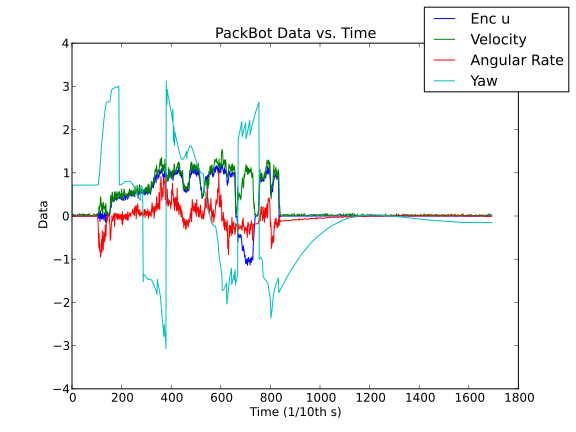
\includegraphics[width=.8\textwidth]{images/pbDataReverseHeading}
	\caption{Heading and Velocity Reversed}
	\label{fig:pbDataReverseHeading}
\end{figure}

*** Figure \ref{fig:pbDataReverseHeading} used encoders and GPS for linear velocity measurements, Microstrain and GPS for heading measurements and Microstrain for yaw rate measurement. The Kalman filter output for heading and the GPS velocity measurements can be seen to flip $180^\circ$ when the robot starts to drive in reverse but the encoders accurately measure the direction of the velocity vector. During the time that the robot is driving in reverse the yaw rate stays slightly negative so the yaw value should be decreasing slightly. The robot drives in reverse from about $65 s - 76s$ as noted in the image. ***

\subsection{Additional Sensors}
\label{sec:kfAdditionalSensors}
*** Talk about adding the compass and using encoder data. ***

\section{Identifty IMU Parameters}
\label{sec:identifyimuparams}
*** Looking at \cite{ChungOjeda01}. Would need access to a rotary table to perform tests. Also look at \cite{ParkinsonHeadingEstimation01} for better estimation of heading. ***
